%%%%%%%%%%%%%%%%%%%%%%%%%%%%%%%%%%%%%%%%%
% Beamer Presentation
% LaTeX Template
% Version 1.0 (10/11/12)
%
% This template has been downloaded from:
% http://www.LaTeXTemplates.com
%
% License:
% CC BY-NC-SA 3.0 (http://creativecommons.org/licenses/by-nc-sa/3.0/)
%
%%%%%%%%%%%%%%%%%%%%%%%%%%%%%%%%%%%%%%%%%

%----------------------------------------------------------------------------------------
%    PACKAGES AND THEMES
%----------------------------------------------------------------------------------------

\documentclass[]{beamer}

\mode<presentation> {

\usetheme{CambridgeUS}

}

\usepackage{graphicx} % Allows including images
\usepackage{url}
\usepackage{hyperref}
\usepackage{amsthm}
\usepackage{tikz}
\usepackage{pifont}

\DeclareGraphicsExtensions{.png, .jpg, .pdf}

\DeclareMathOperator{\poly}{poly}

\setlength{\parskip}{1em}

%----------------------------------------------------------------------------------------
%    TITLE PAGE
%----------------------------------------------------------------------------------------

\title[The Travelling Salesman Problem]{Quantum Speedup of the Travelling Salesman Problem for Bounded Degree Graphs} % The short title appears at the bottom of every slide, the full title is only on the title page

\author[Dominic J. Moylett]{Dominic J. Moylett\footnote{Work completed in collaboration with Ashley Montanaro and Noah Linden.}} % Your name
\institute[University of Bristol] % Your institution as it will appear on the bottom of every slide, may be shorthand to save space
{
School of Physics and Department of Electrical and Electronic Engineering\\
Quantum Engineering Centre for Doctoral Training\\
University of Bristol \\ % Your institution for the title page
\medskip
\textit{\href{mailto:dominic.moylett@bristol.ac.uk}{dominic.moylett@bristol.ac.uk}} % Your email address
}
\date{\today} % Date, can be changed to a custom date

\begin{document}

\begin{frame}
\titlepage % Print the title page as the first slide
\end{frame}

%----------------------------------------------------------------------------------------
%    PRESENTATION SLIDES
%----------------------------------------------------------------------------------------

%------------------------------------------------
\section{Introduction}
%------------------------------------------------

\begin{frame}
\frametitle{Based on a True Story}
\begin{columns}[T]
\begin{column}{.5\textwidth}
I graduated in June 2015.

To celebrate, I wanted to do a tour of Europe.
\end{column}
\begin{column}{.5\textwidth}
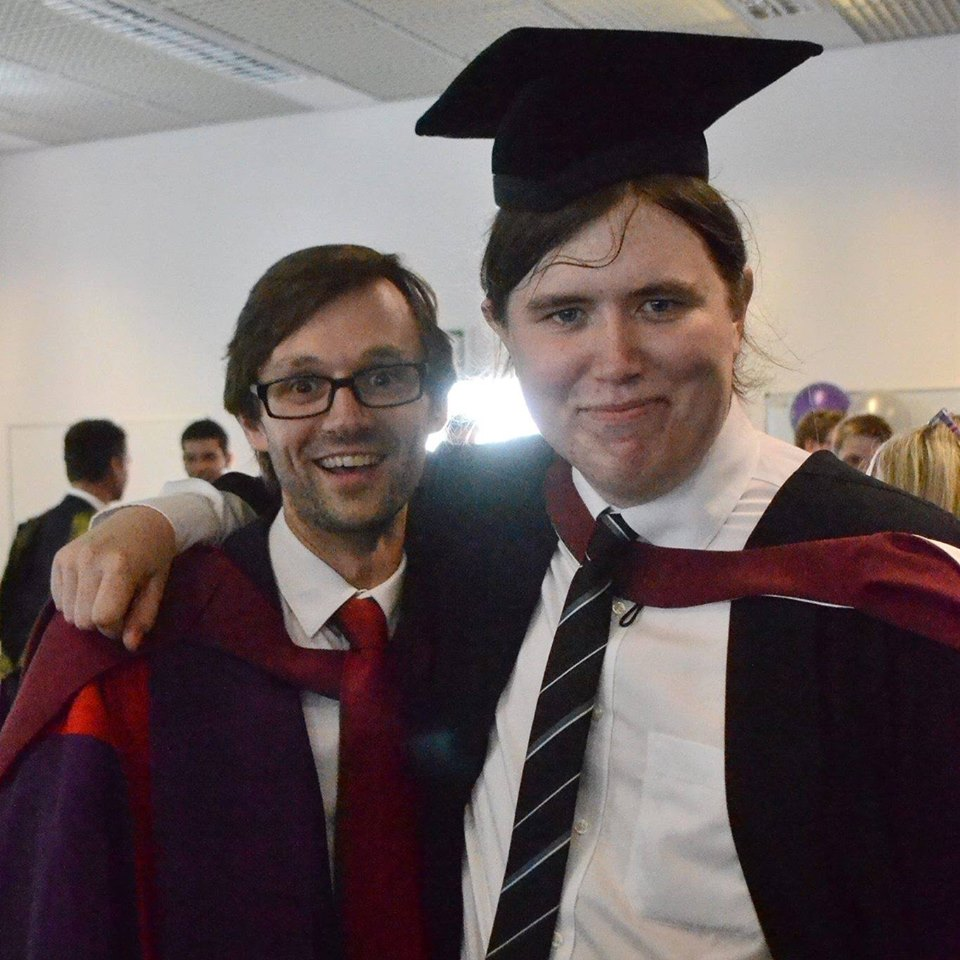
\includegraphics[scale=0.15]{graduation}
\end{column}
\end{columns}
\end{frame}

\begin{frame}
\frametitle{Interrail}
\begin{center}
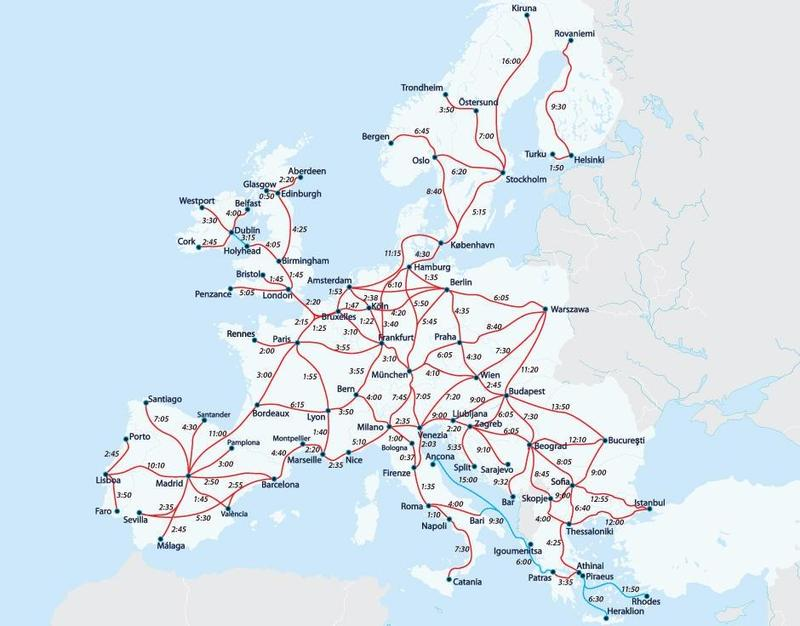
\includegraphics[scale=0.35]{interrail}\footnote{\url{http://www.interrail.eu/plan-your-trip/interrail-railway-map}}
\end{center}
\end{frame}

\begin{frame}
\frametitle{The Grand Tour}
\begin{center}
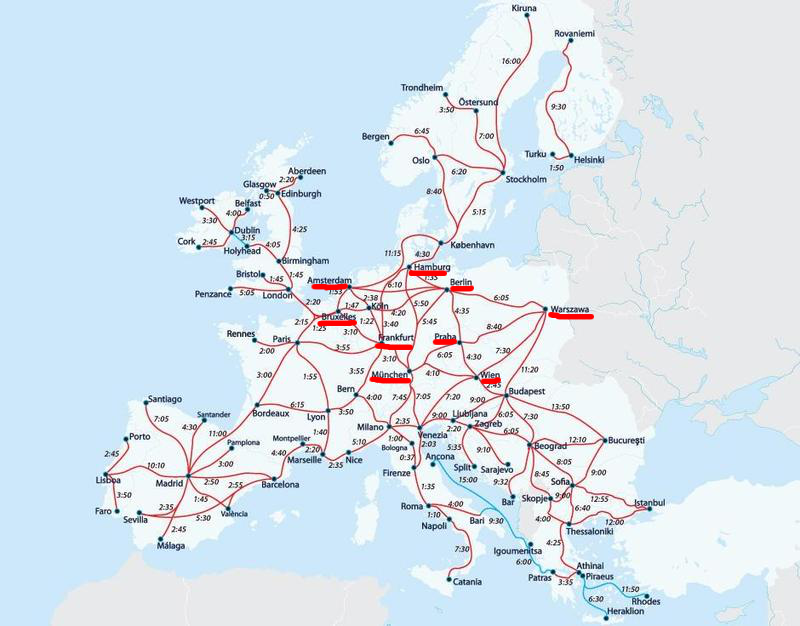
\includegraphics[scale=0.25]{interrail_selected}
\end{center}
What's the fastest way of visiting every location?
\end{frame}

\begin{frame}
\frametitle{The Travelling Salesman Problem}
Given a graph $G = (V, E)$ with cost matrix $C$, what is the Hamiltonian cycle with the lowest cost?

While route finding is the oldest instance of the problem, there are a number of other applications, such as circuit board drilling\footnote{{\em Zeitschrift f{\"u}r Operations Research}, {\bf 35}(61) (1991)}.
\end{frame}

\begin{frame}
\frametitle{Example}
\begin{center}
\begin{tikzpicture}
\path(0,0) node(Amsterdam){Amsterdam} (2,1) node(Hamburg){Hamburg} (4,0) node(Berlin){Berlin} (2,2) node(Copenhagen){Copenhagen} (0,-1) node(Brussels){Brussels} (6,-1) node(Warsaw){Warsaw} (2,-2) node(Frankfurt){Frankfurt} (4,-2) node(Prague){Prague} (2,-3) node(Munich){Munich} (4,-3) node(Vienna){Vienna};

\draw (Amsterdam) -- node[left]{11.25} (Copenhagen);
\draw (Amsterdam) -- node[above]{6.17} (Berlin);
\draw (Amsterdam) -- node[left]{1.88} (Brussels);
\draw (Brussels) -- node[above]{3.17} (Frankfurt);
\draw (Frankfurt) -- node[left]{3.17} (Munich);
\draw (Munich) -- node[above]{6.08} (Prague);
\draw (Munich) -- node[below]{4.17} (Vienna);
\draw (Prague) -- node[]{4.58} (Berlin);
\draw (Prague) -- node[]{4.5} (Vienna);
\draw (Berlin) -- node[above]{6.08} (Warsaw);
\draw (Prague) -- node[above]{8.67} (Warsaw);
\draw (Vienna) -- node[below]{7.5} (Warsaw);
\draw (Hamburg) -- node[right]{4.5} (Copenhagen);
\draw (Berlin) -- node[right]{1.58} (Hamburg);
\end{tikzpicture}

Our example graph.
\end{center}
\end{frame}

\begin{frame}
\frametitle{Example}
\begin{center}
\begin{tikzpicture}
\path(0,0) node(Amsterdam){Amsterdam} (2,1) node(Hamburg){Hamburg} (4,0) node(Berlin){Berlin} (2,2) node(Copenhagen){Copenhagen} (0,-1) node(Brussels){Brussels} (6,-1) node(Warsaw){Warsaw} (2,-2) node(Frankfurt){Frankfurt} (4,-2) node(Prague){Prague} (2,-3) node(Munich){Munich} (4,-3) node(Vienna){Vienna};

\draw (Amsterdam) -- node[left]{11.25} (Copenhagen);
\draw[line width=1.5pt] (Amsterdam) -- node[above]{6.17} (Berlin);
\draw[line width=1.5pt] (Amsterdam) -- node[left]{1.88} (Brussels);
\draw[line width=1.5pt] (Brussels) -- node[above]{3.17} (Frankfurt);
\draw[line width=1.5pt] (Frankfurt) -- node[left]{3.17} (Munich);
\draw (Munich) -- node[above]{6.08} (Prague);
\draw[line width=1.5pt] (Munich) -- node[below]{4.17} (Vienna);
\draw[line width=1.5pt] (Prague) -- node[]{4.58} (Berlin);
\draw[line width=1.5pt] (Prague) -- node[]{4.5} (Vienna);
\draw (Berlin) -- node[above]{6.08} (Warsaw);
\draw (Prague) -- node[above]{8.67} (Warsaw);
\draw (Vienna) -- node[below]{7.5} (Warsaw);
\draw (Hamburg) -- node[right]{4.5} (Copenhagen);
\draw (Berlin) -- node[right]{1.58} (Hamburg);
\end{tikzpicture}

\ding{55} Not a Hamiltonian cycle.
\end{center}
\end{frame}

\begin{frame}
\frametitle{Example}
\begin{center}
\begin{tikzpicture}
\path(0,0) node(Amsterdam){Amsterdam} (2,1) node(Hamburg){Hamburg} (4,0) node(Berlin){Berlin} (2,2) node(Copenhagen){Copenhagen} (0,-1) node(Brussels){Brussels} (6,-1) node(Warsaw){Warsaw} (2,-2) node(Frankfurt){Frankfurt} (4,-2) node(Prague){Prague} (2,-3) node(Munich){Munich} (4,-3) node(Vienna){Vienna};

\draw[line width=1.5pt] (Amsterdam) -- node[left]{11.25} (Copenhagen);
\draw (Amsterdam) -- node[above]{6.17} (Berlin);
\draw[line width=1.5pt] (Amsterdam) -- node[left]{1.88} (Brussels);
\draw[line width=1.5pt] (Brussels) -- node[above]{3.17} (Frankfurt);
\draw[line width=1.5pt] (Frankfurt) -- node[left]{3.17} (Munich);
\draw[line width=1.5pt] (Munich) -- node[above]{6.08} (Prague);
\draw (Munich) -- node[below]{4.17} (Vienna);
\draw (Prague) -- node[]{4.58} (Berlin);
\draw[line width=1.5pt] (Prague) -- node[]{4.5} (Vienna);
\draw[line width=1.5pt] (Berlin) -- node[above]{6.08} (Warsaw);
\draw (Prague) -- node[above]{8.67} (Warsaw);
\draw[line width=1.5pt] (Vienna) -- node[below]{7.5} (Warsaw);
\draw[line width=1.5pt] (Hamburg) -- node[right]{4.5} (Copenhagen);
\draw[line width=1.5pt] (Berlin) -- node[right]{1.58} (Hamburg);
\end{tikzpicture}

\ding{55} Not the shortest Hamiltonian cycle.
\end{center}
\end{frame}

\begin{frame}
\frametitle{Example}
\begin{center}
\begin{tikzpicture}
\path(0,0) node(Amsterdam){Amsterdam} (2,1) node(Hamburg){Hamburg} (4,0) node(Berlin){Berlin} (2,2) node(Copenhagen){Copenhagen} (0,-1) node(Brussels){Brussels} (6,-1) node(Warsaw){Warsaw} (2,-2) node(Frankfurt){Frankfurt} (4,-2) node(Prague){Prague} (2,-3) node(Munich){Munich} (4,-3) node(Vienna){Vienna};

\draw[line width=1.5pt] (Amsterdam) -- node[left]{11.25} (Copenhagen);
\draw (Amsterdam) -- node[above]{6.17} (Berlin);
\draw[line width=1.5pt] (Amsterdam) -- node[left]{1.88} (Brussels);
\draw[line width=1.5pt] (Brussels) -- node[above]{3.17} (Frankfurt);
\draw[line width=1.5pt] (Frankfurt) -- node[left]{3.17} (Munich);
\draw (Munich) -- node[above]{6.08} (Prague);
\draw[line width=1.5pt] (Munich) -- node[below]{4.17} (Vienna);
\draw (Prague) -- node[]{4.58} (Berlin);
\draw[line width=1.5pt] (Prague) -- node[]{4.5} (Vienna);
\draw[line width=1.5pt] (Berlin) -- node[above]{6.08} (Warsaw);
\draw[line width=1.5pt] (Prague) -- node[above]{8.67} (Warsaw);
\draw (Vienna) -- node[below]{7.5} (Warsaw);
\draw[line width=1.5pt] (Hamburg) -- node[right]{4.5} (Copenhagen);
\draw[line width=1.5pt] (Berlin) -- node[right]{1.58} (Hamburg);
\end{tikzpicture}

\ding{51} Solution to the Travelling Salesman Problem.
\end{center}
\end{frame}

\begin{frame}
\frametitle{Difficulty of the Travelling Salesman Problem}
The Travelling Salesman Problem is $NP$-hard, so finding a polynomial time solution would prove that $P = NP$.

A na\"ive solution would take $O(|V|!)$ time by searching over every permutation of the vertices.

D\"urr and H\o yer's quantum algorithm for minimum finding\footnote{{\tt arXiv:quant-ph/9607014}} could be applied to this approach to achieve $O(\sqrt{|V|!})$ time.

But other more efficient classical algorithms exist. Can these be sped up using quantum algorithms?
\end{frame}

\begin{frame}
\frametitle{Our Results}
\begin{itemize}
\item A quadratic speedup for the Travelling Salesman Problem when the degree of any vertex in the graph is at most $3$.
\item This is using a classical algorithm by Eppstein\footnote{{\em Journal of Graph Algorithms and Applications}, {\bf 11}(1), pp.\ 61--81 (2007)}, combined with a quantum speedup by Montanaro\footnote{{\tt arXiv:1509.02374}}.
\item Speedups for graphs of higher bounded degrees are found by reducing to this case.
\end{itemize}
\end{frame}

%------------------------------------------------
\section{How to not speed up the Travelling Salesman Problem}
%------------------------------------------------

\begin{frame}
\frametitle{The Difficulty of a Quantum Speedup}

Key components for many algorithms have limited quantum speedup:

\begin{itemize}
\item The Held-Karp algorithm\footnote{{\em Journal of the Society for Industrial and Applied Mathematics}, {\bf 10}(1), pp.\ 196-210 (1962)} relies on dynamic programming (no known speedup).
\item Christofides' algorithm\footnote{{\em Management Sciences Research Report 388, Graduate School of Industrial Administration, CMU} (1976)} relies on finding a minimum weight perfect matching (polynomial speedup for bipartite graphs).
\item Algorithms which use Nearest Neighbour can be sped up from $O(|V|^2)$ to $O(|V|^{3/2})$ time via minimum finding.
\end{itemize}

Other algorithms do not even have known performance\footnote{{\em Science}, {\bf 220}(4598), pp.\ 671--680 (1983)}.
\end{frame}

%------------------------------------------------
\section{Travelling Salesman Problem on Cubic Graphs}
%------------------------------------------------

\begin{frame}
\frametitle{Eppstein's Algorithm}
Solves the Travelling Salesman Problem when the degree of any vertex is at most $3$.

It takes as input a graph $G = (V, E)$ and a set $F \subseteq E$ of ``forced'' edges and returns the shortest Hamiltonian cycle which includes every edge in $F$.

Main steps:
\begin{enumerate}
\item Reduce $(G, F)$ to $(G', F')$ by changing specific subgraphs in $G$.
\item If $F'$ contains a Hamiltonian cycle then return $F'$.
\item If a Hamiltonian cycle cannot be made, then abort.
\item If $G \setminus F$ is a collection of disjoint cycles of length four then solve and return.
\item Pick an edge $xy \in E' \setminus F'$ according to specific rules.
\item Call Eppstein's algorithm on $(G', F' \cup \{xy\})$ and $(G' \setminus \{xy\}, F')$.
\item Return the shortest Hamiltonian cycle or abort if no cycle is found.
\end{enumerate}
\end{frame}

\begin{frame}
\frametitle{Edge Picking}
The main bottleneck of Eppstein's algorithm is the recursive calls. So how is the edge to force or remove chosen?

\begin{enumerate}
\item If $G' \setminus F'$ has a cycle of four vertices such that two of the vertices are incident to forced edges, pick one vertex $x$ in the cycle that is not incident to a forced edge and another vertex $y$ not in the cycle.
\item Otherwise if $F' \neq \emptyset$, pick an edge $(y, z) \in F$ and then chooses an adjacent edge $(x, y) \notin F$ as long as $(x, y)$ is not part of a disjoint cycle of four vertices in $G \setminus F$.
\item Otherwise pick any edge.
\end{enumerate}

\end{frame}

\begin{frame}
\frametitle{Performance}
Eppstein showed that these branching rules broke the problem size into one of two cases:

\begin{enumerate}
\item A subproblem with two more forced edges and one more cycle of $4$ unforced edges, and a subproblem with three fewer vertices.
\item Two subproblems with at least three more forced edges.
\item A subproblem with at least two more forced edges, and a subproblem with at least five more forced edges.
\end{enumerate}

Linear recurrence solving shows that the overall runtime is $O(2^{n/3})$.
\end{frame}

\begin{frame}
\frametitle{Example Recursion}
\begin{tikzpicture}[scale=0.75]
\tikzstyle{vertex}=[draw,shape=circle]
\path (0,0) node[vertex](f0){};
\path (-2,-1) node[vertex](x0){} (-1,-2) node[vertex](x1){} (0,-1) node[vertex](f1){} (1,-2) node[vertex](y1){} (2,-1) node[vertex](y0){};
\path (-1,-3) node[vertex](x2){} (1,-3) node[vertex](y2){};
\path (-3,0) node[vertex](x3){} (-1,0) node[vertex](x4){};
\draw[line width=1.5pt] (f0) -- (f1);
\draw[line width=1.5pt] (x2) -- (x1);
\draw (x0) -- (x1) -- node[above]{$x$} (f1) -- node[above]{$y$} (y1) -- (y2);
\draw (x3) -- (x0) -- (x4);
\draw (y0) -- (y1);

\path (-5,-5) node[vertex](f0){};
\path (-7,-6) node[vertex](x0){} (-6,-7) node[vertex](x1){} (-5,-6) node[vertex](f1){} (-4,-7) node[vertex](y1){} (-3,-6) node[vertex](y0){};
\path (-6,-8) node[vertex](x2){} (-4,-8) node[vertex](y2){};
\path (-8,-5) node[vertex](x3){} (-6,-5) node[vertex](x4){};
\draw[line width=1.5pt] (f0) -- (f1) -- node[above]{$y$} (y1);
\draw[line width=1.5pt] (x0) -- (x1) -- (x2);
\draw (x3) -- (x0) -- (x4);
\draw (y0) -- (y1) -- (y2);

\path (5,-5) node[vertex](f0){};
\path (3,-6) node[vertex](x0){} (4,-7) node[vertex](x1){} (5,-6) node[vertex](f1){} (6,-7) node[vertex](y1){} (7,-6) node[vertex](y0){};
\path (4,-8) node[vertex](x2){} (6,-8) node[vertex](y2){};
\path (2,-5) node[vertex](x3){} (4,-5) node[vertex](x4){};
\draw[line width=1.5pt] (f0) -- (f1) -- node[above]{$x$} (x1) -- (x2);
\draw[line width=1.5pt] (x3) -- (x0) -- (x4);
\draw[line width=1.5pt] (y2) -- (y1) -- (y0);

\draw[thick, ->] (-2,-3) -- (-3,-4);
\draw[thick, ->] (2,-3) -- (3,-4);
\end{tikzpicture}
\end{frame}

\begin{frame}
\frametitle{Why not use minimum finding?}
D\"urr and H\o yer's algorithm for minimum finding can be used if we can map a binary string to each result of the algorithm.

We can map binary strings to Eppstein's algorithm by removing an edge if the next bit is $0$ and forcing it if the next bit is $1$.

However, the longest bit string we might need is $n/2$ bits, because of the case which only adds two forced edges to the graph.

Thus we have a runtime of $O(2^{n/4})$.

We need to take advantage of the problem's structure if we want to do even better.
\end{frame}

\begin{frame}
\frametitle{Backtracking Algorithms}
Backtracking algorithms are algorithms to solve constraint satisfaction problems, where we have $n$ variables to assign values to such that they satisfy $m$ constraints.

They work by using a predicate $P$ and heuristic $h$ as follows, given a partial assigment $V$:

\begin{enumerate}
\item If $P(V) = \top$ then return $V$.
\item Else if $P(V) = \bot$ then abort.
\item Let $v_{i} \leftarrow h(V)$.
\item For all possible values $a$ that we can assign to $v_{i}$:
\begin{enumerate}
\item Call recursively on $(V \cup (v_{i}, a))$ to get assignment $V'$.
\item If call does not abort then return assignment $V'$.
\end{enumerate}
\item Abort.
\end{enumerate}
\end{frame}

\begin{frame}
\frametitle{Quantum Speedup for Backtracking Algorithms}

Montanaro proved the following:

\begin{theorem}[Montanaro]
Let $T$ be the number of recursive calls made by a backtracking algorithm. For any $0 < \delta < 1$, there is a quantum algorithm which evaluates $P$ and $h$ $O(\sqrt{T}n^{3/2}\log(n)\log(1/\delta))$ times, and outputs a partial assignment $V$ such that $P(V)$ is true or aborts if no such $V$ exists. The algorithm fails with probability $\delta$.
\end{theorem}

This speedup works by visualising the backtracking algorithm's calls as a tree and performing a quantum walk on the tree.
\end{frame}

\begin{frame}
\frametitle{Applying Montanaro's Speedup to Eppstein's Algorithm}

Eppstein's algorithm is an example of a backtracking algorithm. The variables are the edges in the graph, of which there are at most $3|V|/2$, and the values we can assign to them are whether an edge is forced or removed.

To fit the framework used by Montanaro's quantum algorithm, we need to rewrite Eppstein's algorithm in terms of the predicate and heuristic functions.
\end{frame}

\begin{frame}
\frametitle{The Predicate}

\begin{enumerate}
\item Apply any already known assignments to the graph.
\item Reduce $(G, F)$ to $(G', F')$ by changing specific subgraphs in $G$.
\item If $F'$ contains a Hamiltonian cycle then return $\top$.
\item If a Hamiltonian cycle cannot be made, then return $\bot$.
\item If $G \setminus F$ is a collection of disjoint cycles of length four then return $\top$.
\item Otherwise return ?
\end{enumerate}
\end{frame}

\begin{frame}
\frametitle{The Heuristic}

\begin{enumerate}
\item Apply any already known assignments to the graph.
\item Reduce $(G, F)$ to $(G', F')$ by changing specific subgraphs in $G$.
\item Pick an edge $xy \in E' \setminus F'$ according to specific rules.
\item If $xy$ is made up of several edges in $E$ then return one of the edges in $xy$.
\item Otherwise return $xy$.
\end{enumerate}
\end{frame}

\begin{frame}
\frametitle{Finding the Shortest Hamiltonian Cycle}

The algorithm as it is currently described will return a randomly chosen Hamiltonian cycle with probability $\delta$ in $O(2^{|V|/6}\poly(|V|)\log(1/\delta))$ time. However, this is not guaranteed to be the shortest Hamiltonian cycle.

To find the shortest Hamiltonian cycle, we will repeat the process, but with the extra condition that the predicate returns $\bot$ if the combined cost of all the cycles in $F'$ is above a threashold $T$. We then use binary search to find the shortest Hamiltonian cycle after $O(\log N)$ calls of the algorithm, where

$$N = \sum_{i = 0}^{n-1}\max_{j = 0}^{n-1}\{c_{i,j}\}$$

is an upper bound for the length of any Hamiltonian cycle.
\end{frame}

\begin{frame}
\frametitle{Quantum Speedup on Cubic Graphs}
\begin{theorem}
There is a quantum algorithm which solves the TSP for graphs of bounded degree $3$ with probability $\delta$ in time $O(\log N2^{n/6}\poly(n)\log(\log N/\delta))$.
\end{theorem}
\end{frame}

%------------------------------------------------
\section{Towards Higher Degrees}
%------------------------------------------------

\begin{frame}
\frametitle{Beyond Cubic Graphs}
After achieving a speedup for cubic graphs, we looked at whether or not graphs of higher degree could also be sped up.

This is done through two components:
\begin{enumerate}
\item Reducing the graph to instances of lower degree graphs.
\item Speeding up the search over these lower degree instances via D\"urr and H\o yer's algorithm for minimum finding.
\end{enumerate}
\end{frame}

\begin{frame}
\frametitle{Degree $4$ Vertices}

There are three ways we can split a degree $4$ vertex into two vertices of degree $3$ connected by a forced edge:

\begin{center}
\begin{tikzpicture}[scale=0.9]
\tikzstyle{vertex}=[draw,shape=circle]
\path (0,0) node[vertex](x1){} (1,0) node[vertex](y1){};
\draw[line width=1.5pt] (x1) -- (y1);
\draw[] (-1,1) -- node[above] {$a$} (x1);
\draw[] (-1,-1) -- node[above] {\textbf{$b$}} (x1);
\draw[] (y1) -- node[above] {$c$} (2,1);
\draw[] (y1) -- node[above] {$d$} (2,-1);

\path (4,0) node[vertex](x1){} (5,0) node[vertex](y1){};
\draw[line width=1.5pt] (x1) -- (y1);
\draw[] (3,1) -- node[above] {$a$} (x1);
\draw[] (3,-1) -- node[above] {$c$} (x1);
\draw[] (y1) -- node[above] {$b$} (6,1);
\draw[] (y1) -- node[above] {$d$} (6,-1);

\path (8,0) node[vertex](x1){} (9,0) node[vertex](y1){};
\draw[line width=1.5pt] (x1) -- (y1);
\draw[] (7,1) -- node[above] {$a$} (x1);
\draw[] (7,-1) -- node[above] {$d$} (x1);
\draw[] (y1) -- node[above] {$c$} (10,1);
\draw[] (y1) -- node[above] {$b$} (10,-1);
\end{tikzpicture}
\end{center}

If $a$ and $b$ are the two edges which are part of the shortest Hamiltonian cycle, there are two ways of splitting the vertex which preserve the answer.
\end{frame}

\begin{frame}
\frametitle{Bounded Degree $4$ Graphs}
Let $k$ be the number of degree $4$ vertices in the graph.

There are $3^k$ ways of reducing the graph to a degree $3$ graph which we can solve, of which $2^k$ will have the shortest Hamiltonian cycle.

Note that this splitting does increase the number of vertices, but it also increases the number of forced edges, so the problem size as a whole does not increase.

By applying D\"urr and H\o yer's algorithm for minimum finding, we can find the shortest Hamiltonian cycle after $(3/2)^{k/2}$ repeated calls. Thus our runtime is

$$O\left(\left(\frac{3}{2}\right)^{\frac{k}{2}}\log N2^{\frac{n}{3}}\poly(n)\log\left(\frac{\log N}{\delta}\right)\right).$$
\end{frame}

\begin{frame}
\frametitle{Bounded Degree $4$ Graphs}

Since $k \leq n$, we can bound this and work out the runtime to be

$$O(1.375^n\log N\poly(n)\log(\log N/\delta)).$$

This beats the best known classical runtime of $O(1.692^n)$ by Xiao and Nagamochi\footnote{{\em Theory of Computing Systems}, {\bf 58}(2), pp.\ 241--272 (2016)}.
\end{frame}

\begin{frame}
\frametitle{Degree $5$ Vertices}

There are ten ways we can split a degree $5$ vertex into a vertex of degree $4$ and another of degree $3$ connected by a forced edge:

\begin{center}
\begin{tikzpicture}[scale=0.55]
\tikzstyle{vertex}=[draw,shape=circle]
\path (0,0) node[vertex](x1){} (1,0) node[vertex](y1){};
\draw[line width=1.5pt] (x1) -- (y1);
\draw[] (-1,1) -- node[above] {$a$} (x1);
\draw[] (-1,0) -- node[above] {$b$} (x1);
\draw[] (-1,-1) -- node[above] {$c$} (x1);
\draw[] (y1) -- node[above] {$d$} (2,1);
\draw[] (y1) -- node[above] {$e$} (2,0);

\path (4,0) node[vertex](x1){} (5,0) node[vertex](y1){};
\draw[line width=1.5pt] (x1) -- (y1);
\draw[] (3,1) -- node[above] {$a$} (x1);
\draw[] (3,0) -- node[above] {$b$} (x1);
\draw[] (3,-1) -- node[above] {$d$} (x1);
\draw[] (y1) -- node[above] {$c$} (6,1);
\draw[] (y1) -- node[above] {$e$} (6,0);

\path (8,0) node[vertex](x1){} (9,0) node[vertex](y1){};
\draw[line width=1.5pt] (x1) -- (y1);
\draw[] (7,1) -- node[above] {$a$} (x1);
\draw[] (7,0) -- node[above] {$b$} (x1);
\draw[] (7,-1) -- node[above] {$e$} (x1);
\draw[] (y1) -- node[above] {$c$} (10,1);
\draw[] (y1) -- node[above] {$d$} (10,0);

\path (12,0) node[vertex](x1){} (13,0) node[vertex](y1){};
\draw[line width=1.5pt] (x1) -- (y1);
\draw[] (11,1) -- node[above] {$a$} (x1);
\draw[] (11,0) -- node[above] {$b$} (x1);
\draw[] (y1) -- node[above] {$c$} (14,1);
\draw[] (y1) -- node[above] {$d$} (14,0);
\draw[] (y1) -- node[above] {$e$} (14,-1);

\path (16,0) node[vertex](x1){} (17,0) node[vertex](y1){};
\draw[line width=1.5pt] (x1) -- (y1);
\draw[] (15,1) -- node[above] {$a$} (x1);
\draw[] (15,0) -- node[above] {$c$} (x1);
\draw[] (15,-1) -- node[above] {$d$} (x1);
\draw[] (y1) -- node[above] {$b$} (18,1);
\draw[] (y1) -- node[above] {$e$} (18,0);

\path (0,-3) node[vertex](x1){} (1,-3) node[vertex](y1){};
\draw[line width=1.5pt] (x1) -- (y1);
\draw[] (-1,-2) -- node[above] {$a$} (x1);
\draw[] (-1,-3) -- node[above] {$c$} (x1);
\draw[] (-1,-4) -- node[above] {$e$} (x1);
\draw[] (y1) -- node[above] {$b$} (2,-2);
\draw[] (y1) -- node[above] {$d$} (2,-3);

\path (4,-3) node[vertex](x1){} (5,-3) node[vertex](y1){};
\draw[line width=1.5pt] (x1) -- (y1);
\draw[] (3,-2) -- node[above] {$a$} (x1);
\draw[] (3,-3) -- node[above] {$c$} (x1);
\draw[] (y1) -- node[above] {$b$} (6,-2);
\draw[] (y1) -- node[above] {$d$} (6,-3);
\draw[] (y1) -- node[above] {$e$} (6,-4);

\path (8,-3) node[vertex](x1){} (9,-3) node[vertex](y1){};
\draw[line width=1.5pt] (x1) -- (y1);
\draw[] (7,-2) -- node[above] {$a$} (x1);
\draw[] (7,-3) -- node[above] {$d$} (x1);
\draw[] (7,-4) -- node[above] {$e$} (x1);
\draw[] (y1) -- node[above] {$b$} (10,-2);
\draw[] (y1) -- node[above] {$c$} (10,-3);

\path (12,-3) node[vertex](x1){} (13,-3) node[vertex](y1){};
\draw[line width=1.5pt] (x1) -- (y1);
\draw[] (11,-2) -- node[above] {$a$} (x1);
\draw[] (11,-3) -- node[above] {$d$} (x1);
\draw[] (y1) -- node[above] {$b$} (14,-2);
\draw[] (y1) -- node[above] {$c$} (14,-3);
\draw[] (y1) -- node[above] {$e$} (14,-4);

\path (16,-3) node[vertex](x1){} (17,-3) node[vertex](y1){};
\draw[line width=1.5pt] (x1) -- (y1);
\draw[] (15,-2) -- node[above] {$a$} (x1);
\draw[] (15,-3) -- node[above] {$e$} (x1);
\draw[] (y1) -- node[above] {$b$} (18,-2);
\draw[] (y1) -- node[above] {$c$} (18,-3);
\draw[] (y1) -- node[above] {$d$} (18,-4);
\end{tikzpicture}
\end{center}

If $a$ and $b$ are the two edges which are part of the shortest Hamiltonian cycle, there are six ways of splitting the vertex which preserve the answer.
\end{frame}

\begin{frame}
\frametitle{Bounded Degree $5$ Graphs}
There are $10^k$ ways of reducing the graph to a bounded degree $4$ graph, of which $6^k$ will have the shortest Hamiltonian cycle.

By using the same techniques as before, we get a runtime of

$$O\left(\left(\frac{10}{6}\right)^{\frac{k}{2}}1.375^n\log N\poly(n)\log\left(\frac{\log N}{\delta}\right)\right).$$
\end{frame}

\begin{frame}
\frametitle{Bounded Degree $5$ Graphs}

Since $k \leq n$, we can bound this and work out the runtime to be

$$O(1.775^n\log N\poly(n)\log(\log N/\delta)).$$

This beats the best known classical runtime by Bj\"orklund et al.\ of $O(1.932^n\poly(n))$\footnote{{\em Proceedings of the 35th International Colloquium on Automata, Languages and Programming}, pp.\ 198--209 (2008)}.
\end{frame}

\begin{frame}
\frametitle{Degree $6$ Vertices}

There are ten ways we can split a degree $6$ vertex into two vertices of degree $4$ connected by a forced edge:

\begin{center}
\begin{tikzpicture}[scale=0.55]
\tikzstyle{vertex}=[draw,shape=circle]
\path (0,0) node[vertex](x1){} (1,0) node[vertex](y1){};
\draw[line width=1.5pt] (x1) -- (y1);
\draw[] (-1,1) -- node[above] {$a$} (x1);
\draw[] (-1,0) -- node[above] {$b$} (x1);
\draw[] (-1,-1) -- node[above] {$c$} (x1);
\draw[] (y1) -- node[above] {$d$} (2,1);
\draw[] (y1) -- node[above] {$e$} (2,0);
\draw[] (y1) -- node[above] {$f$} (2,-1);

\path (4,0) node[vertex](x1){} (5,0) node[vertex](y1){};
\draw[line width=1.5pt] (x1) -- (y1);
\draw[] (3,1) -- node[above] {$a$} (x1);
\draw[] (3,0) -- node[above] {$b$} (x1);
\draw[] (3,-1) -- node[above] {$d$} (x1);
\draw[] (y1) -- node[above] {$c$} (6,1);
\draw[] (y1) -- node[above] {$e$} (6,0);
\draw[] (y1) -- node[above] {$f$} (6,-1);

\path (8,0) node[vertex](x1){} (9,0) node[vertex](y1){};
\draw[line width=1.5pt] (x1) -- (y1);
\draw[] (7,1) -- node[above] {$a$} (x1);
\draw[] (7,0) -- node[above] {$b$} (x1);
\draw[] (7,-1) -- node[above] {$e$} (x1);
\draw[] (y1) -- node[above] {$c$} (10,1);
\draw[] (y1) -- node[above] {$d$} (10,0);
\draw[] (y1) -- node[above] {$f$} (10,-1);

\path (12,0) node[vertex](x1){} (13,0) node[vertex](y1){};
\draw[line width=1.5pt] (x1) -- (y1);
\draw[] (11,1) -- node[above] {$a$} (x1);
\draw[] (11,0) -- node[above] {$b$} (x1);
\draw[] (11,-1) -- node[above] {$f$} (x1);
\draw[] (y1) -- node[above] {$c$} (14,1);
\draw[] (y1) -- node[above] {$d$} (14,0);
\draw[] (y1) -- node[above] {$e$} (14,-1);

\path (16,0) node[vertex](x1){} (17,0) node[vertex](y1){};
\draw[line width=1.5pt] (x1) -- (y1);
\draw[] (15,1) -- node[above] {$a$} (x1);
\draw[] (15,0) -- node[above] {$c$} (x1);
\draw[] (15,-1) -- node[above] {$d$} (x1);
\draw[] (y1) -- node[above] {$b$} (18,1);
\draw[] (y1) -- node[above] {$e$} (18,0);
\draw[] (y1) -- node[above] {$f$} (18,-1);

\path (0,-3) node[vertex](x1){} (1,-3) node[vertex](y1){};
\draw[line width=1.5pt] (x1) -- (y1);
\draw[] (-1,-2) -- node[above] {$a$} (x1);
\draw[] (-1,-3) -- node[above] {$c$} (x1);
\draw[] (-1,-4) -- node[above] {$e$} (x1);
\draw[] (y1) -- node[above] {$b$} (2,-2);
\draw[] (y1) -- node[above] {$d$} (2,-3);
\draw[] (y1) -- node[above] {$f$} (2,-4);

\path (4,-3) node[vertex](x1){} (5,-3) node[vertex](y1){};
\draw[line width=1.5pt] (x1) -- (y1);
\draw[] (3,-2) -- node[above] {$a$} (x1);
\draw[] (3,-3) -- node[above] {$c$} (x1);
\draw[] (3,-4) -- node[above] {$f$} (x1);
\draw[] (y1) -- node[above] {$b$} (6,-2);
\draw[] (y1) -- node[above] {$d$} (6,-3);
\draw[] (y1) -- node[above] {$e$} (6,-4);

\path (8,-3) node[vertex](x1){} (9,-3) node[vertex](y1){};
\draw[line width=1.5pt] (x1) -- (y1);
\draw[] (7,-2) -- node[above] {$a$} (x1);
\draw[] (7,-3) -- node[above] {$d$} (x1);
\draw[] (7,-4) -- node[above] {$e$} (x1);
\draw[] (y1) -- node[above] {$b$} (10,-2);
\draw[] (y1) -- node[above] {$c$} (10,-3);
\draw[] (y1) -- node[above] {$f$} (10,-4);

\path (12,-3) node[vertex](x1){} (13,-3) node[vertex](y1){};
\draw[line width=1.5pt] (x1) -- (y1);
\draw[] (11,-2) -- node[above] {$a$} (x1);
\draw[] (11,-3) -- node[above] {$d$} (x1);
\draw[] (11,-4) -- node[above] {$f$} (x1);
\draw[] (y1) -- node[above] {$b$} (14,-2);
\draw[] (y1) -- node[above] {$c$} (14,-3);
\draw[] (y1) -- node[above] {$e$} (14,-4);

\path (16,-3) node[vertex](x1){} (17,-3) node[vertex](y1){};
\draw[line width=1.5pt] (x1) -- (y1);
\draw[] (15,-2) -- node[above] {$a$} (x1);
\draw[] (15,-3) -- node[above] {$e$} (x1);
\draw[] (15,-4) -- node[above] {$f$} (x1);
\draw[] (y1) -- node[above] {$b$} (18,-2);
\draw[] (y1) -- node[above] {$c$} (18,-3);
\draw[] (y1) -- node[above] {$d$} (18,-4);
\end{tikzpicture}
\end{center}

If $a$ and $b$ are the two edges which are part of the shortest Hamiltonian cycle, there are six ways of splitting the vertex which preserve the answer.
\end{frame}

\begin{frame}
\frametitle{Bounded Degree $6$ Graphs}
As we have the same splitting results as we had for bounded degree $5$, we have the same runtime of $O(1.775^n\log N\poly(n)\log(\log N/\delta))$.

This beats the best known classical time by Bj\"orklund et al.\ of $O(1.967^n\poly(n))$.
\end{frame}

\begin{frame}
\frametitle{Bounded Degree $7$}
There are $\binom{7}{4} = 35$ ways of splitting a vertex of degree $7$ into one vertex of degree $5$ and another of degree $4$ connected by a forced edge. Of these, $35 - \binom{4}{2} - \binom{5}{2} = 26$ will succeed. Thus we achieve a runtime of

\begin{align*}
&O\left(\left(\frac{35}{26}\right)^{k/2}1.768^n\log N\poly(n)\log\left(\frac{1}{\delta}\right)\right)\\
= &O(2.0513^n\log N\poly(n)\log(1/\delta)).
\end{align*}

Thus we are no longer beating Bj{\"o}rklund et al., which has a runtime of $O(1.9840^n\poly(n))$.
\end{frame}

%------------------------------------------------
\section{Next Steps}
%------------------------------------------------

\begin{frame}
\frametitle{Faster Algorithms}
Eppstein's algorithm was the first backtracking algorithm to solve the Travelling Salesman Problem. But other backtracking algorithms have faster runtimes:

\begin{itemize}
\item Iwama and Nakashima\footnote{13th Annual International Conference on Computing and Combinatorics, pp.\ 108--117 (2007)} have an algorithm for bounded degree $3$ graphs which runs in $O(1.251^n)$ time.
\item Li\'{s}kiewicz and Schuster\footnote{{\em Journal of Discrete Algorithms}, {\bf 27}, pp.\ 1--20 (2014)} have an algorithm for bounded degree $3$ graphs which runs in $O(1.2553^n)$ time and challenge the result of Iwama and Nakashima.
\item Xiao and Nagamochi\footnote{{\em Algorithmica}, {\bf 74}(2), pp.\ 713--741 (2016)}\footnote{{\em Theory of Computing Systems}, {\bf 58}(2), pp.\ 241--272 (2016)} have given runtimes of $O(1.2312^n)$ and $O(1.692^n)$ for graphs of bounded degree $3$ and $4$, respectively.
\end{itemize}
\end{frame}

%------------------------------------------------
\section{Conclusion}
%------------------------------------------------

\begin{frame}
\frametitle{Conclusion}
The Travelling Salesman Problem is one of the most famous problems in all of Computer Science.

We have demonstrated quantum speedups for the Travelling Salesman Problem for graphs where the degree of any vertex is at most $6$.

Future Steps:
\begin{itemize}
\item Apply further analysis to algorithms by Xiao and Nagamochi to see if we can yield an even better quantum speedup.
\item ???
\item Publish!
\end{itemize}
\end{frame}

%------------------------------------------------
\section{The End}
%------------------------------------------------

\begin{frame}
\frametitle{The End}
\begin{center}
Any questions?

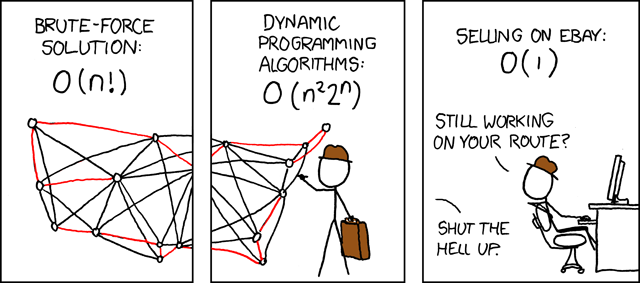
\includegraphics[scale=0.5]{xkcd}\footnote{\url{https://xkcd.com/399/}}
\end{center}
\end{frame}

%------------------------------------------------
\section{Post-credits}
%------------------------------------------------

\begin{frame}
\frametitle{Post-credits}
\centerline{This is not the slide you're looking for.}
\end{frame}

%----------------------------------------------------------------------------------------

\end{document} 
